\let\negmedspace\undefined
\let\negthickspace\undefined
\documentclass[journal]{IEEEtran}
\usepackage[a5paper, margin=10mm, onecolumn]{geometry}
%\usepackage{lmodern} % Ensure lmodern is loaded for pdflatex
\usepackage{tfrupee} % Include tfrupee package

\setlength{\headheight}{1cm} % Set the height of the header box
\setlength{\headsep}{0mm}     % Set the distance between the header box and the top of the text

\usepackage{gvv-book}
\usepackage{gvv}
\usepackage{cite}
\usepackage{amsmath,amssymb,amsfonts,amsthm}
\usepackage{algorithmic}
\usepackage{graphicx}
\usepackage{textcomp}
\usepackage{xcolor}
\usepackage{txfonts}
\usepackage{listings}
\usepackage{enumitem}
\usepackage{mathtools}
\usepackage{gensymb}
\usepackage{comment}
\usepackage[breaklinks=true]{hyperref}
\usepackage{tkz-euclide} 
\usepackage{listings}
% \usepackage{gvv}                                        
\def\inputGnumericTable{}                                 
\usepackage[latin1]{inputenc}                                
\usepackage{color}                                            
\usepackage{array}                                            
\usepackage{longtable}                                       
\usepackage{calc}                                             
\usepackage{multirow}                                         
\usepackage{hhline}                                           
\usepackage{ifthen}                                           
\usepackage{lscape}
\begin{document}

\bibliographystyle{IEEEtran}
\vspace{3cm}

\title{4.2.15}
\author{EE24BTECH11041 - Mohit}
% \maketitle
% \newpage
% \bigskip
{\let\newpage\relax\maketitle}

\renewcommand{\thefigure}{\theenumi}
\renewcommand{\thetable}{\theenumi}
\setlength{\intextsep}{10pt} % Space between text and floats


\numberwithin{equation}{enumi}
\numberwithin{figure}{enumi}
\renewcommand{\thetable}{\theenumi}

\begin{enumerate}
\item Find the direction and normal vectors of the line $y=2x$ . \\
SOLUTION
\begin{table}[h!]    
  \centering
  \begin{tabular}[12pt]{ |c| c| c| c| c| c|}
    \hline
    x & 1 & 2 & 3 & 4 & 5 \\ 
    \hline
    y & 14 & 13 & 9 & 5 & 2 \\
    \hline   
    \end{tabular}

  \caption{Variables Used}
  \label{tab 1.4.9.2}
\end{table}
\begin{align}
	y = 2x \\
	\leftrightarrow y = mx + c \\
	A &= \myvec{1 \\ m} = \myvec{1 \\ 2} \\
	B &= \myvec{ -m \\ 1 } = \myvec{ -2 \\ 1 } 
\end{align}
where $\vec{A}$ and $\vec{B}$ denote the Direction and Normal vectors of the line respectively.
\begin{align}
	\vec{A} = \myvec{ 1 \\ 2} \\
	\vec{B} = \myvec{ -2 \\ 1} 
\end{align}
\end{enumerate}
\begin{figure}[h!]
   \centering
   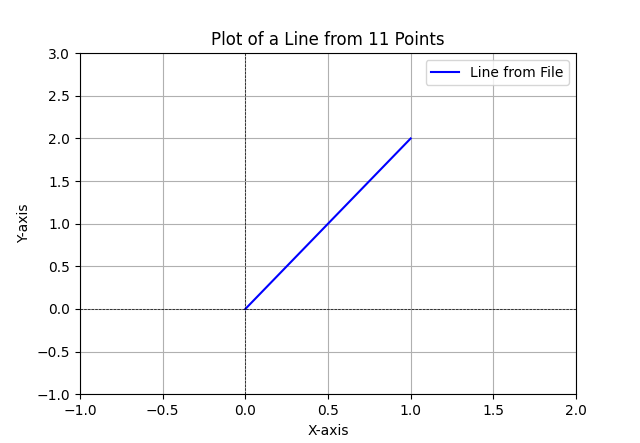
\includegraphics[width=0.7\linewidth]{figs/Figure_1.png}
   \caption{Equation of Line  $ABC$}
   \label{stemplot}
\end{figure}
\end{document}
